
\chapter{Experiments and Results}\label{chap:experiments}

This chapter evaluates the pipeline described in Chapter~\ref{chap:methodology}. Instead of presenting the results as a disconnected list of scores, the chapter is organised around five experimental questions. Each question corresponds to one main design choice in the pipeline:

\begin{enumerate}
\item Which OCR engine reads nutrition labels most accurately?
(Section~\ref{sec:exp-ocr})
\item Which semantic classifier detects nutrient entities most reliably?
(Section~\ref{sec:exp-classifier})
\item Which association engine builds better tuples, graph~v1 or
graph~v2? (Section~\ref{sec:exp-assoc})
\item If a vision--language model is used only at the association step,
does it perform better than the graph-based association method, and
how does it compare with a fully end-to-end vision--language model
that maps the image directly to tuples?
(Section~\ref{sec:exp-vlm})
\item Which edge-creation mode performs best inside graph~v2?
(Section~\ref{sec:exp-edge})
\end{enumerate}

The first two questions focus on the OCR and semantic classification stages. The last three questions all relate to the association stage, but they examine it from different perspectives: the choice of graph engine, the possible use of a vision--language model for association, and the effect of the edge-creation mode inside graph~v2.

To answer these questions, 14 pipeline configurations were evaluated. In each experiment, the pipeline is kept unchanged except for the component being tested. This allows changes in performance to be linked to the stage under investigation, rather than to unrelated changes elsewhere in the system. Figure~\ref{fig:ablation-tree} presents the full experimental design as a single ablation tree and serves as the map for the rest of this chapter. Each leaf represents one experiment. The path leading to that leaf shows the OCR engine, classifier, association engine, and edge mode used in that configuration, while the value at the leaf reports the four-field tuple F1 score (4F-F1).

The dataset, annotation schema, evaluation metrics, and tuple-matching procedure were already defined in Chapter~\ref{chap:evaluation}, so they are not repeated here. Unless stated otherwise, the term ``best'' refers to the highest 4F-F1 score. However, not every experimental question can be answered by this score alone. For example, the OCR comparison also considers per-field accuracy, the classifier comparison reports nutrient-field metrics, and the graph and vision--language experiments additionally examine performance on single-context and multi-context images. When precision or recall changes the interpretation of a ranking, the corresponding section reports these values separately.
\begin{figure}[p]
  \centering
  \makebox[\textwidth][c]{%
    \includegraphics[width=1.2\textwidth,height=1.1\textheight,keepaspectratio]%
      {ablation_tree_portrait.png}%
  }
  \caption[Ablation results tree]{%
Summary tree of the 14 ablation experiments. Each path shows the OCR
engine, classifier, association method, and, for graph~v2, the
edge-creation mode. Leaves report 4F-F1. Border styles indicate
interpretability tiers, colours distinguish OCR engines, amber marks
graph~v2 edge-mode variants, the filled diamond marks the best edge
mode, and the star marks the best fully interpretable pipeline.}

  \label{fig:ablation-tree}
\end{figure}
% =====================================================================
%  6.1  EXPERIMENTAL SETUP
% =====================================================================
\section{Experimental Setup}\label{sec:exp-setup}

This section records the configuration held fixed across the experiments
and lists the runs. The dataset, the annotation schema, the four-field
(4F) and three-field (3F) tuple metrics, and the tuple-matching procedure
used for scoring are defined in Chapter~\ref{chap:evaluation} and are
reused here without restatement. Every result in this chapter is produced
by the same evaluator on the test set of 57 labelled images and 866 gold
tuples, so all scores are directly comparable.

The fixed backbone is as follows. PaddleOCR PP-OCRv5 is the OCR engine for
every run except the EasyOCR baseline used to settle the OCR axis
(Section~\ref{sec:exp-ocr}). When graph~v2 is the association engine it
uses the \mcode{overlap} edge mode, with default row, column, and context
overlap thresholds of 0.30, 0.20, and 0.10. The two learned classifiers
run at fixed, calibrated operating points---GLiNER-biomed at its selected
score threshold and the BGE-M3 embedding classifier at its selected
threshold and margin---which are reported in
Section~\ref{sec:exp-classifier}. The vision--language model used at the
association step and end to end is Gemma~3~4B Instruct.

All scoring is done by the evaluator of Chapter~\ref{chap:evaluation}. It
is fully reproducible, returning the same scores on every run, so the
comparison across runs is exact. The primary metric is the four-field
tuple F1 (4F-F1), the share of gold tuples whose nutrient, quantity,
unit, and context are all correct; the three-field tuple F1 (3F-F1),
which drops the context field, is reported alongside it where it adds
information.

Table~\ref{tab:exp-registry} lists the runs used in this chapter. Each run
is named by the label used throughout, and is defined by its OCR engine,
classifier, association engine, and (for graph~v2) edge mode; the headline
column is its four-field tuple F1. The four additional graph~v2
edge-mode variants used only in Section~\ref{sec:exp-edge} are introduced
there and are not listed here.

\begin{table}[htbp]
  \centering
  \caption[Experiment registry]{The runs used in this chapter. Each run is
    identified by the label used throughout and is defined by its OCR
    engine, semantic classifier, association engine, and graph~v2 edge
    mode. The run \mbox{E2-A} is the PaddleOCR rule-based reference,
    also referred to as EXP-02. Two 4F-F1 columns are given: the full test
    set (866 tuples, 57 images) and the reduced set
    (820~tuples, 55~images) with images 15 and 67 removed, as defined in
    Chapter~\ref{chap:evaluation}. The remaining metrics appear in the
    indicated sections and are reported on the full set.}
  \label{tab:exp-registry}
  \small
  \begin{tabular}{@{}llllccc@{}}
    \toprule
     & & & & & \multicolumn{2}{c}{\textbf{4F-F1}} \\
    \cmidrule(lr){6-7}
    \textbf{ID} & \textbf{OCR} & \textbf{Classifier} & \textbf{Association} & \textbf{Edge mode} & \textbf{Full (866)} & \textbf{Reduced (820)} \\
    \midrule
    EXP-01          & EasyOCR    & Rule-based & Graph~v2       & \mcode{overlap} & 0.1773 & 0.1833 \\
    \addlinespace
    E2-A            & PaddleOCR  & Rule-based & Graph~v2       & \mcode{overlap} & 0.4231 & 0.4262 \\
    E2-B            & PaddleOCR  & Embedding  & Graph~v2       & \mcode{overlap} & 0.4025 & 0.4049 \\
    E2-C            & PaddleOCR  & GLiNER     & Graph~v2       & \mcode{overlap} & 0.4304 & 0.4341 \\
    \addlinespace
    E3-EMB-G1       & PaddleOCR  & Embedding  & Graph~v1       & ---             & 0.2325 & 0.2392 \\
    E3-GLiNER-G1    & PaddleOCR  & GLiNER     & Graph~v1       & ---             & 0.2523 & 0.2599 \\
    \addlinespace
    A\_VLM          & PaddleOCR  & Rule-based & VLM assoc.\    & ---             & 0.4819 & 0.4944 \\
    E3-EMB-VLM      & PaddleOCR  & Embedding  & VLM assoc.\    & ---             & 0.4945 & 0.5092 \\
    E3-GLiNER-VLM   & PaddleOCR  & GLiNER     & VLM assoc.\    & ---             & 0.4446 & 0.4555 \\
    \addlinespace
    E4              & ---        & ---        & End-to-end VLM & ---             & 0.3597 & 0.3704 \\
    \bottomrule
  \end{tabular}
\end{table}

The two columns track together. Removing images 15 and 67 raises every run
slightly---between 0.002 and 0.015 in four-field F1---and changes no
position in the ranking: E3-EMB-VLM stays highest overall, E2-C stays the
best fully interpretable run, and EXP-01 stays lowest. The gains are small
because both removed images were among the weakest in the set. The rest of
this chapter reports on the full set of 866 tuples; the reduced column is
given here so the two test sets can be compared directly.

% =====================================================================
%  6.2  OCR AXIS
% =====================================================================
\section{OCR Engine}\label{sec:exp-ocr}

The first question is which OCR engine reads the labels best. Two engines
are compared: EasyOCR and PaddleOCR PP-OCRv5. Everything after the OCR
stage is held fixed---the rule-based classifier, graph~v2 with the
\mcode{overlap} edge mode, and the same association and evaluation
steps---so any difference in the score comes from the OCR engine alone.
This axis is settled first, because OCR quality limits every later stage,
and the winning engine is then used for the rest of the chapter. The two
runs are EXP-01 (EasyOCR) and E2-A (PaddleOCR), also called EXP-02.

The OCR engine is not measured by the tuple score alone. Its real job is
to deliver tokens that the later stages can read correctly, so the first
table reports per-field accuracy: how often the nutrient, quantity, unit,
and context are correct once a nutrient has been matched.
Table~\ref{tab:ocr-fields} shows these numbers.

\begin{table}[htbp]
  \centering
  \caption[OCR axis: field-level results]{Field-level results for the two
    OCR engines, with the downstream pipeline held fixed (rule-based
    classifier, graph~v2, \mcode{overlap}). Nutrient detection is reported
    as precision, recall, and F1; the quantity, unit, and context fields
    are reported as accuracy over matched nutrients. PaddleOCR wins every
    field.}
  \label{tab:ocr-fields}
  \small
  \begin{tabular}{@{}lcccccc@{}}
    \toprule
     & \multicolumn{3}{c}{\textbf{Nutrient}} & \textbf{Quantity} & \textbf{Unit} & \textbf{Context} \\
    \cmidrule(lr){2-4}
    \textbf{OCR engine} & P & R & F1 & acc & acc & acc \\
    \midrule
    EasyOCR (EXP-01)    & 0.6667 & 0.6882 & 0.6773 & 0.4547 & 0.5168 & 0.6141 \\
    PaddleOCR (E2-A)    & 0.7227 & 0.7252 & 0.7239 & 0.7691 & 0.8121 & 0.8726 \\
    \addlinespace
    \textbf{Difference} & +0.0560 & +0.0370 & +0.0466 & +0.3144 & +0.2953 & +0.2585 \\
    \bottomrule
  \end{tabular}
\end{table}

\begin{figure}[t]
  \centering
  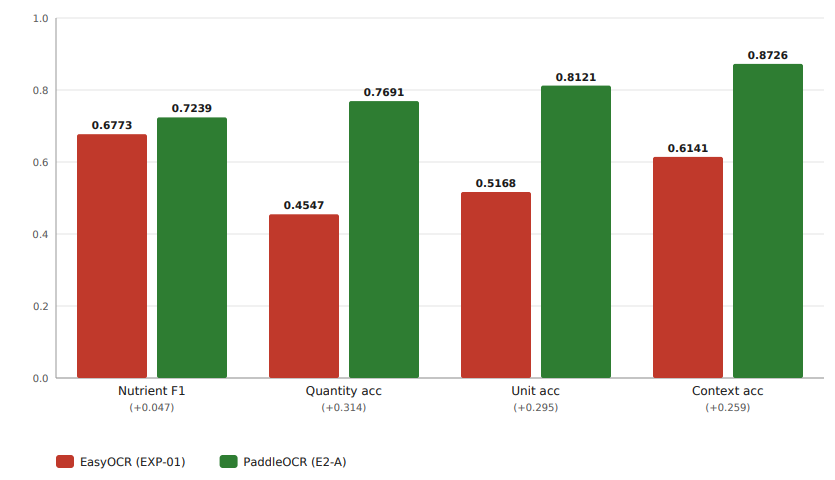
\includegraphics[width=1.2\linewidth,keepaspectratio]{ocr_fields_bars.png}
  \caption[OCR engine: per-field performance]{Per-field performance of the
    two OCR engines, with the downstream pipeline fixed (rule-based
    classifier, graph~v2, \mcode{overlap}). Nutrient is reported as F1;
    quantity, unit, and context as accuracy over matched nutrients. The two
    engines are close on nutrient detection, but PaddleOCR is far ahead on
    quantity, unit, and context---the value fields---which is where the
    full-tuple gain comes from.}
  \label{fig:ocr-fields-bars}
\end{figure}

The pattern is clear. Both engines find nutrient names about equally well:
nutrient recall rises by only about 4~points with PaddleOCR, and EasyOCR
even produces slightly more candidate tokens overall. The large gap is in
reading the values. PaddleOCR improves quantity accuracy by about
31~points, unit accuracy by about 30~points, and context accuracy by
about 26~points. In other words, EasyOCR can locate the text but often
misreads the numbers and short unit tokens, while PaddleOCR reads them
correctly. This matters because a tuple is only counted when all four
fields are right, so an error in the quantity or unit field is enough to
lose the tuple even when the nutrient name was found.

The full-tuple scores in Table~\ref{tab:ocr-tuple} follow directly from
this. The per-field gains in quantity, unit, and context combine, and the
four-field tuple F1 more than doubles, from 0.1773 to 0.4231.

\begin{table}[htbp]
  \centering
  \caption[OCR axis: full-tuple results]{Full-tuple results for the two
    OCR engines, downstream fixed. Scores are reported for the
    three-field tuple (3F, nutrient--quantity--unit) and the four-field
    tuple (4F, including context), each as precision, recall, and F1.}
  \label{tab:ocr-tuple}
  \small
  \begin{tabular}{@{}lcccccc@{}}
    \toprule
     & \multicolumn{3}{c}{\textbf{3F (n,q,u)}} & \multicolumn{3}{c}{\textbf{4F (n,q,u,x)}} \\
    \cmidrule(lr){2-4}\cmidrule(lr){5-7}
    \textbf{OCR engine} & P & R & F1 & P & R & F1 \\
    \midrule
    EasyOCR (EXP-01)    & 0.2327 & 0.2402 & 0.2364 & 0.1745 & 0.1801 & 0.1773 \\
    PaddleOCR (E2-A)    & 0.4407 & 0.4423 & 0.4415 & 0.4223 & 0.4238 & 0.4231 \\
    \bottomrule
  \end{tabular}
\end{table}

The conclusion of this axis is that PaddleOCR PP-OCRv5 is the stronger
engine, and the gain comes from reading quantities and units rather than
from finding more nutrient names. PaddleOCR is therefore fixed as the OCR
engine for all remaining experiments in this chapter.

% =====================================================================
%  6.3  CLASSIFIER AXIS
% =====================================================================
\section{Semantic Classifier}\label{sec:exp-classifier}

The second question is which semantic classifier detects nutrients best.
Three classifiers are compared: the rule-based lexicon, the BGE-M3
embedding classifier, and GLiNER-biomed. PaddleOCR is now fixed, and the
rest of the pipeline is held constant (graph~v2 with the \mcode{overlap}
edge mode), so any difference comes from the classifier. The three runs
are E2-A (rule-based), E2-B (embedding), and E2-C (GLiNER).
Figure~\ref{fig:classified-tokens} shows the embedding classifier's token
labels on two example labels, each coloured by its predicted role.

\begin{figure}[htbp]
  \centering
  \begin{minipage}[t]{0.330\textwidth}
    \centering
    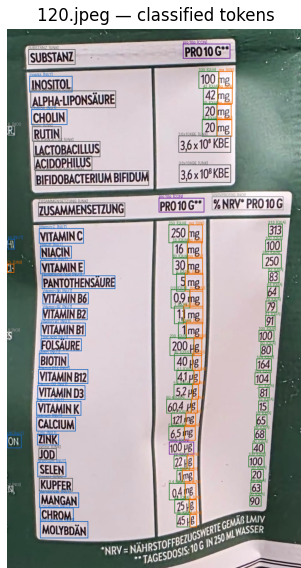
\includegraphics[width=\linewidth]{classified_tokens_120.png}\\[3pt]
    {\small (a)}
  \end{minipage}\hfill
  \begin{minipage}[t]{0.610\textwidth}
    \centering
    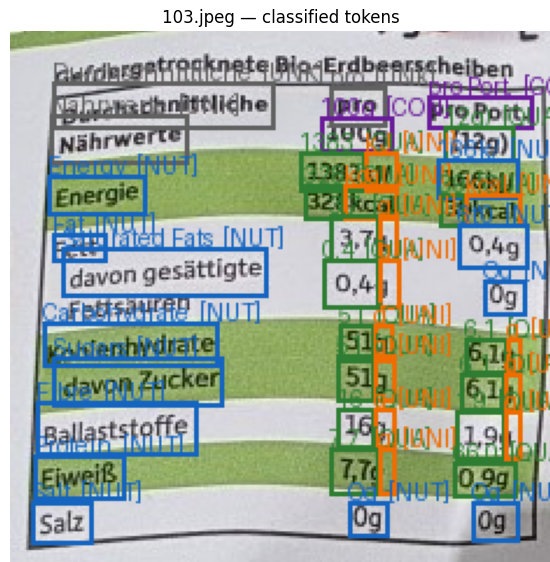
\includegraphics[width=\linewidth]{classified_tokens_103.png}\\[3pt]
    {\small (b)}
  \end{minipage}
  \caption[Classified tokens from the embedding classifier]{%
    Token classification produced by the BGE-M3 embedding classifier on two
    example labels: (a)~a dense supplement panel (120.jpeg) and (b)~a standard
    nutrition table (103.jpeg). Each detected token is boxed and coloured by its
    predicted role --- nutrient (blue), quantity (green), unit (orange), and
    context (purple). The four roles are the four scored tuple fields.}
  \label{fig:classified-tokens}
\end{figure}

One point must be made before the numbers, because it decides how this
axis is read. The three classifiers share the entire deterministic
cascade described in Section~\ref{sec:classifier-cascade}. Quantity,
unit, context, NRV, and noise are all resolved by that shared cascade and
are identical across the three runs. The only thing that changes is the
final nutrient / not-nutrient decision. The classifier axis is therefore
measured directly on the nutrient field; the quantity, unit, and context
fields are reported as well, but any movement in them is an indirect
effect of a different nutrient set changing which rows the graph builds,
not the classifier acting on those fields.

Table~\ref{tab:classifier-fields} shows this. The nutrient field is given
as precision, recall, and F1; the other three fields are given as
accuracy. The nutrient numbers move by several points across the three
classifiers, while the quantity, unit, and context accuracies stay within
about two points of each other---direct evidence that the shared cascade,
not the classifier, owns those fields.

\begin{table}[htbp]
  \centering
  \caption[Classifier axis: field-level results]{Field-level results for
    the three classifiers, with OCR fixed to PaddleOCR and the downstream
    pipeline fixed (graph~v2, \mcode{overlap}). The nutrient field is
    reported as precision, recall, and F1; quantity, unit, and context
    are reported as accuracy over matched nutrients. The nutrient field is
    the only one the classifier controls; the other three are resolved by
    the shared deterministic cascade and barely change.}
  \label{tab:classifier-fields}
  \small
  \begin{tabular}{@{}lcccccc@{}}
    \toprule
     & \multicolumn{3}{c}{\textbf{Nutrient}} & \textbf{Quantity} & \textbf{Unit} & \textbf{Context} \\
    \cmidrule(lr){2-4}
    \textbf{Classifier} & P & R & F1 & acc & acc & acc \\
    \midrule
    Rule-based (E2-A) & 0.7227 & 0.7252 & 0.7239 & 0.7691 & 0.8121 & 0.8726 \\
    Embedding (E2-B)  & 0.6580 & 0.6975 & 0.6771 & 0.7649 & 0.8311 & 0.8642 \\
    GLiNER (E2-C)     & 0.7350 & 0.6374 & 0.6827 & 0.7627 & 0.8315 & 0.8786 \\
    \bottomrule
  \end{tabular}
\end{table}

The three classifiers behave differently on the nutrient field. The
rule-based lexicon has the highest nutrient recall, 0.7252, because the
labels in this dataset are largely covered by its curated entries; its
weakness is that it is closed-vocabulary by construction. Among the two
learned classifiers, the embedding classifier has the higher recall,
0.6975 against GLiNER's 0.6374, because it accepts candidates by semantic
similarity rather than exact coverage and so recovers nutrient names that
GLiNER's threshold rejects. The cost of that recall is precision: the
embedding classifier has the lowest nutrient precision, 0.6580, so it also
admits the most non-nutrient tokens. GLiNER is the opposite---the highest
nutrient precision, 0.7350, and the lowest recall.

These thresholds were set by the token-level calibration described in
Section~\ref{sec:classifier-embedding} and
Section~\ref{sec:classifier-gliner}. The embedding classifier runs at a
cosine threshold of 0.59 with a margin of 0.04, where its token-level
nutrient F1 is about 0.87. GLiNER runs at a span threshold of 0.18, where
its token-level nutrient F1 is about 0.89, with precision 0.91 and recall
0.87. The rule-based classifier has no threshold; it accepts a candidate
when the lexicon or one of its supporting rules matches.

The full-tuple ranking in Table~\ref{tab:classifier-tuple} is the
downstream consequence of these nutrient decisions passing through the
fixed cascade and the fixed graph. GLiNER gives the best four-field F1,
0.4304, followed by the rule-based classifier at 0.4231 and the embedding
classifier at 0.4025.

\begin{table}[htbp]
  \centering
  \caption[Classifier axis: full-tuple ranking]{Full-tuple ranking of the
    three classifiers, OCR and downstream fixed. Scores are the
    three-field tuple (3F) and four-field tuple (4F), each as precision,
    recall, and F1. Rows are ordered by 4F-F1.}
  \label{tab:classifier-tuple}
  \small
  \begin{tabular}{@{}lcccccc@{}}
    \toprule
     & \multicolumn{3}{c}{\textbf{3F (n,q,u)}} & \multicolumn{3}{c}{\textbf{4F (n,q,u,x)}} \\
    \cmidrule(lr){2-4}\cmidrule(lr){5-7}
    \textbf{Classifier} & P & R & F1 & P & R & F1 \\
    \midrule
    GLiNER (E2-C)     & 0.4807 & 0.4169 & 0.4465 & 0.4634 & 0.4018 & 0.4304 \\
    Rule-based (E2-A) & 0.4407 & 0.4423 & 0.4415 & 0.4223 & 0.4238 & 0.4231 \\
    Embedding (E2-B)  & 0.4085 & 0.4330 & 0.4204 & 0.3911 & 0.4145 & 0.4025 \\
    \bottomrule
  \end{tabular}
\end{table}

The reason GLiNER wins on the tuple score even though it does not have the
best nutrient recall is precision. Its high nutrient precision means few
non-nutrient tokens enter the graph, so few false-positive tuples are
produced, and it has the highest four-field precision, 0.4634. The
embedding classifier shows the opposite effect. Its surplus nutrient
candidates are passed to the graph, which binds them into tuples without
re-checking whether they are real, so they become false-positive tuples.
This gives the embedding classifier the lowest four-field precision,
0.3911, and the lowest four-field F1, even though its nutrient recall is
higher than GLiNER's. This precision penalty is specific to the graph
association engine; Section~\ref{sec:exp-vlm} shows that it disappears when
the vision--language model handles association, which is where the
embedding classifier's recall becomes an advantage.

For the rest of the chapter, GLiNER is treated as the main zero-shot
classifier, because it gives the best interpretable tuple score without a
manually curated lexicon. The embedding classifier is kept as the second
zero-shot variant, and the rule-based classifier as a strong
closed-vocabulary reference.



% =====================================================================
%  6.4  ASSOCIATION AXIS — GRAPH V1 vs GRAPH V2
% =====================================================================
\section{Association Engine: Graph v1 versus Graph v2}\label{sec:exp-assoc}

The third question is which association engine builds better tuples. This
section compares the two graph engines of Chapter~\ref{chap:methodology},
graph~v1 (Section~\ref{sec:graph-v1}) and graph~v2
(Section~\ref{sec:graph-v2}). OCR is fixed to PaddleOCR, and the
\mcode{overlap} edge mode is used for graph~v2. The comparison is run with
the two learned, zero-shot classifiers, embedding and GLiNER, since these
are the classifiers used with both graph engines; the graph~v2 results for
all three classifiers were already given in Section~\ref{sec:exp-classifier}.
The four runs are E3-EMB-G1 and E2-B for embedding, and E3-GLiNER-G1 and
E2-C for GLiNER.

Table~\ref{tab:graph-tuple} gives the full-tuple results. The effect is
large and is the same for both classifiers: graph~v2 nearly doubles the
four-field F1 of graph~v1, from 0.2325 to 0.4025 for embedding and from
0.2523 to 0.4304 for GLiNER. Because the jump appears for both classifiers,
it comes from the graph engine, not from the classifier.

\begin{table}[htbp]
  \centering
  \caption[Graph v1 versus graph v2: full-tuple results]{Full-tuple
    results for graph~v1 and graph~v2, with OCR fixed to PaddleOCR and the
    \mcode{overlap} edge mode used for graph~v2. Scores are the
    three-field tuple (3F) and four-field tuple (4F), each as precision,
    recall, and F1.}
  \label{tab:graph-tuple}
  \small
  \begin{tabular}{@{}llcccccc@{}}
    \toprule
     & & \multicolumn{3}{c}{\textbf{3F (n,q,u)}} & \multicolumn{3}{c}{\textbf{4F (n,q,u,x)}} \\
    \cmidrule(lr){3-5}\cmidrule(lr){6-8}
    \textbf{Classifier} & \textbf{Association} & P & R & F1 & P & R & F1 \\
    \midrule
    Embedding & Graph v1 (E3-EMB-G1)    & 0.3277 & 0.3591 & 0.3427 & 0.2223 & 0.2436 & 0.2325 \\
    Embedding & Graph v2 (E2-B)         & 0.4085 & 0.4330 & 0.4204 & 0.3911 & 0.4145 & 0.4025 \\
    \addlinespace
    GLiNER    & Graph v1 (E3-GLiNER-G1) & 0.3923 & 0.3510 & 0.3705 & 0.2671 & 0.2390 & 0.2523 \\
    GLiNER    & Graph v2 (E2-C)         & 0.4807 & 0.4169 & 0.4465 & 0.4634 & 0.4018 & 0.4304 \\
    \bottomrule
  \end{tabular}
\end{table}

The table also shows where the gain is. The three-field score, which
covers only nutrient, quantity, and unit, improves moderately from
graph~v1 to graph~v2. The four-field score, which adds context, improves
much more. For embedding, the gap between the 3F and 4F score is 0.110
under graph~v1 but only 0.018 under graph~v2; for GLiNER it falls from
0.118 to 0.016. In other words, graph~v1 loses many tuples on the context
field, and graph~v2 almost closes that gap. The context field is where
graph~v2 makes the difference.

The field-level numbers in Table~\ref{tab:graph-fields} confirm this. Going
from graph~v1 to graph~v2, quantity and unit accuracy improve by about 7
to 9~points, but context accuracy improves by about 25~points for
embedding and 27~points for GLiNER. The context field moves several times
more than the others.

\begin{table}[htbp]
  \centering
  \caption[Graph v1 versus graph v2: field accuracy]{Field accuracy for
    graph~v1 and graph~v2, over matched nutrients. Quantity and unit
    improve moderately, while context improves by about 25 to 27~points.}
  \label{tab:graph-fields}
  \small
  \begin{tabular}{@{}llccc@{}}
    \toprule
    \textbf{Classifier} & \textbf{Association} & \textbf{Quantity} & \textbf{Unit} & \textbf{Context} \\
    \midrule
    Embedding & Graph v1 & 0.6950 & 0.7433 & 0.6150 \\
    Embedding & Graph v2 & 0.7649 & 0.8311 & 0.8642 \\
    \addlinespace
    GLiNER    & Graph v1 & 0.6924 & 0.7624 & 0.6059 \\
    GLiNER    & Graph v2 & 0.7627 & 0.8315 & 0.8786 \\
    \bottomrule
  \end{tabular}
\end{table}



The reason is the way the two graphs handle context. Graph~v1 uses a single
\mcode{CONTEXT_SCOPE} edge that reaches nutrient nodes only, so when a label
has more than one value column it cannot keep the columns apart, and the
wrong context is often attached. Graph~v2 adds the \mcode{HEADER_SCOPE} edge
described in Section~\ref{sec:graph-v2}, which binds each header to the
tokens in its own column. This keeps a per-100\,g column and a per-serving
column separate, so each value receives the context of its own column.

If this explanation is correct, the advantage of graph~v2 should appear
only on labels that actually have more than one context. To test this, the
57 test images are split into 20 single-context images (159 tuples), where
all values share one context, and 37 multi-context images (707 tuples),
where the values span two or more contexts. Table~\ref{tab:graph-context}
reports the four-field recall on each group; recall is used here because
the question is how many of the gold tuples each engine recovers.




\begin{table}[htbp]
  \centering
  \caption[Graph v1 versus graph v2: single- and multi-context recall]{%
    Four-field recall of graph~v1 and graph~v2 on single-context images (20
    images, 159 tuples) and multi-context images (37 images, 707 tuples).
    On single-context images the two engines are almost equal; on
    multi-context images graph~v2 nearly doubles graph~v1.}
  \label{tab:graph-context}
  \small
  \begin{tabular}{@{}llcc@{}}
    \toprule
    \textbf{Classifier} & \textbf{Association} & \textbf{Single-context} & \textbf{Multi-context} \\
    \midrule
    Embedding & Graph v1 & 0.497 & 0.187 \\
    Embedding & Graph v2 & 0.522 & 0.390 \\
    \addlinespace
    GLiNER    & Graph v1 & 0.497 & 0.181 \\
    GLiNER    & Graph v2 & 0.522 & 0.375 \\
    \bottomrule
  \end{tabular}
\end{table}

The split confirms the explanation. On single-context images the two graph
engines are almost equal: recall rises only from 0.497 to 0.522, because
with one context there is nothing for graph~v2 to separate. On
multi-context images graph~v2 nearly doubles graph~v1, from 0.187 to 0.390
for embedding and from 0.181 to 0.375 for GLiNER. The whole advantage of
graph~v2 comes from the multi-context labels, which is exactly what the
\mcode{HEADER_SCOPE} edge was designed to handle. The single-context recall
is also identical for the two classifiers (the same hit counts on both),
which shows that on these simpler layouts the association engine, not the
classifier, is what matters.

% =====================================================================
%  WORKED EXAMPLE — graph v1 vs graph v2 on image 34
%  Placement: inside Section~\ref{sec:exp-assoc}, after the single/multi-context
%  discussion (Table~\ref{tab:graph-context} and the context-recall figure).
%  Needs \usepackage{amssymb} for \checkmark.
%  Figure: 34.png (add your uploaded label image).
% =====================================================================

To make the multi-context advantage concrete, one label is examined in full.
Image~34 is a vitamin and mineral supplement whose table prints every value
twice, once per 100\,g and once per 25\,g serving
(Figure~\ref{fig:example34-label}). The gold set has 40 tuples for this label,
20 under each context. It is a clean instance of the two-column layout described
above: two value columns that share a single column of nutrient names.

\begin{figure}[htbp]
  \centering
  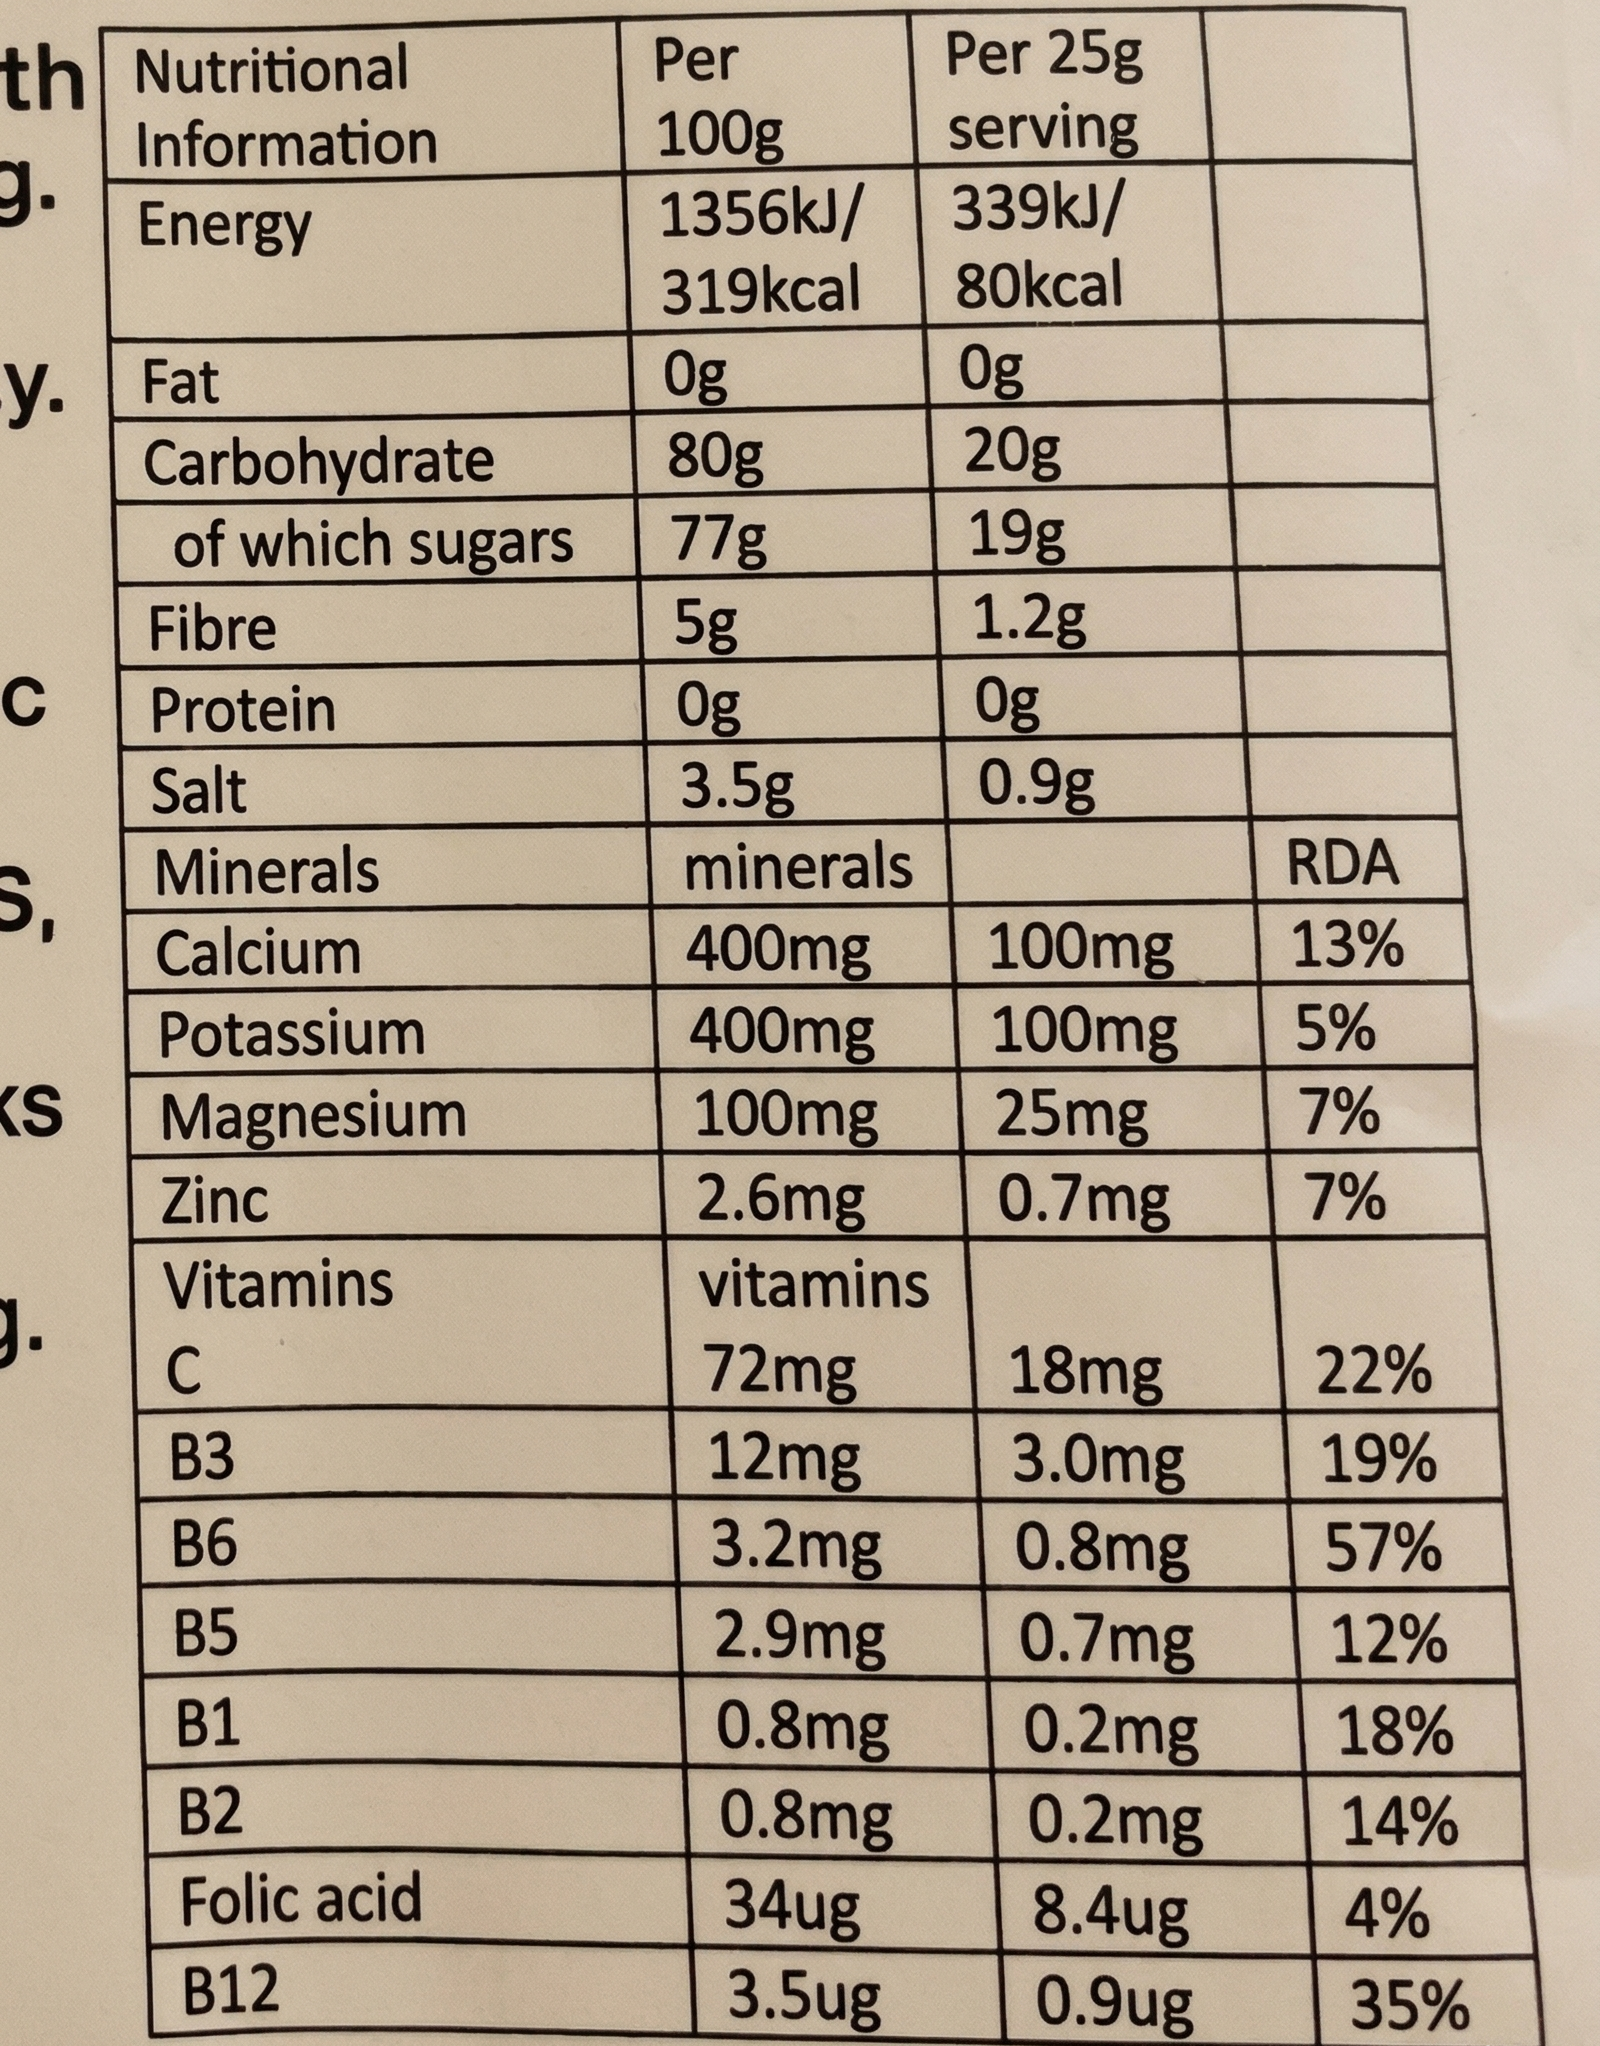
\includegraphics[width=0.60\linewidth,keepaspectratio]{34.png}
  \caption[Image 34: a two-context supplement label]{Image~34. Each nutrient is
    listed once per 100\,g and once per 25\,g serving, so the label has two value
    columns under one column of names. This is the layout where graph~v2's
    \mcode{HEADER_SCOPE} edge keeps the two contexts apart and graph~v1's single
    context edge does not.}
  \label{fig:example34-label}
\end{figure}

Table~\ref{tab:example34} shows the output of the two graph engines on this
label. For every nutrient it marks which of the two contexts each engine
recovers with all four fields correct. Graph~v1 recovers 15 of the 40 tuples,
while graph~v2 recovers 30, exactly double.

\begin{table}[htbp]
  \centering
  \caption[Worked example: correct tuples on image 34]{Correct four-field tuples
    on image~34, by nutrient and context. A check mark means the engine recovers
    that tuple with nutrient, quantity, unit, and context all correct; a blank
    cell means it does not. Each context has 20 gold tuples. Graph~v2 fills both
    columns, while graph~v1 recovers the per-100\,g column but none of the
    per-serving column.}
  \label{tab:example34}
  \small
  \begin{tabular}{@{}lcccc@{}}
    \toprule
     & \multicolumn{2}{c}{\textbf{Per 100\,g}} & \multicolumn{2}{c}{\textbf{Per 25\,g serving}} \\
    \cmidrule(lr){2-3}\cmidrule(lr){4-5}
    \textbf{Nutrient} & \textbf{v1} & \textbf{v2} & \textbf{v1} & \textbf{v2} \\
    \midrule
    Energy (kJ)      &            &            &            &            \\
    Energy (kcal)    &            &            &            &            \\
    Fat              &            & \checkmark &            &            \\
    Carbohydrate     & \checkmark & \checkmark &            & \checkmark \\
    Sugars           & \checkmark & \checkmark &            & \checkmark \\
    Fibre            & \checkmark & \checkmark &            & \checkmark \\
    Protein          & \checkmark & \checkmark &            &            \\
    Salt             & \checkmark & \checkmark &            & \checkmark \\
    Calcium          & \checkmark & \checkmark &            & \checkmark \\
    Potassium        & \checkmark & \checkmark &            & \checkmark \\
    Magnesium        & \checkmark & \checkmark &            & \checkmark \\
    Zinc             & \checkmark & \checkmark &            & \checkmark \\
    Vitamin C        & \checkmark & \checkmark &            & \checkmark \\
    Niacin           & \checkmark & \checkmark &            & \checkmark \\
    Vitamin B6       & \checkmark & \checkmark &            & \checkmark \\
    Pantothenic Acid & \checkmark & \checkmark &            & \checkmark \\
    Vitamin B1       & \checkmark & \checkmark &            & \checkmark \\
    Vitamin B2       & \checkmark & \checkmark &            & \checkmark \\
    Folic Acid       &            &            &            &            \\
    Vitamin B12      &            &            &            &            \\
    \midrule
    \textbf{Recovered (of 20)} & \textbf{15} & \textbf{16} & \textbf{0} & \textbf{14} \\
    \bottomrule
  \end{tabular}
\end{table}

The pattern is clear. On the per-100\,g column the two engines are almost the
same, 15 against 16. On the per-serving column graph~v1 recovers nothing at all,
while graph~v2 recovers 14. Graph~v1 does not fail on the numbers themselves; on
the first column it reads and binds them as well as graph~v2. It fails because
its single \mcode{CONTEXT_SCOPE} edge folds the label into one context, so the
whole per-serving column is left without a correct context and every tuple in it
is lost. Graph~v2 keeps the two columns apart with the \mcode{HEADER_SCOPE} edge
of Section~\ref{sec:graph-v2}, tying each value to the header of its own column,
so the 14 serving tuples are recovered. The gain is not better reading, but
keeping the second context alive.

The same behaviour holds across the whole multi-context set
(Table~\ref{tab:graph-context}); image~34 simply makes it visible. Almost the
entire advantage of graph~v2 on this label is the per-serving column that
graph~v1 drops.

The conclusion of this part of the axis is that graph~v2 is the stronger
association engine, and its advantage is structural: it attaches the
correct context in labels that report nutrients under more than one
reference basis, which graph~v1 cannot do.



\begin{figure}[t]
  \centering
  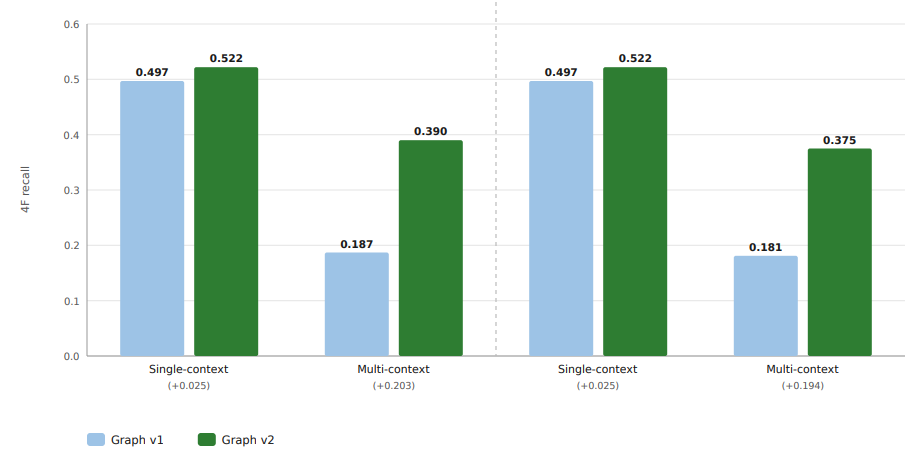
\includegraphics[width=1.2\linewidth,keepaspectratio]{graph_context_bars.png}
  \caption[Graph v1 vs graph v2: recall by context multiplicity]{Four-field
    recall of graph~v1 and graph~v2 on single-context images (159 tuples)
    and multi-context images (707 tuples), for both learned classifiers,
    OCR fixed and \mcode{overlap} edge mode. On single-context images the
    two engines are nearly equal; on multi-context images graph~v2 nearly
    doubles graph~v1. The whole advantage of graph~v2 is on multi-context
    labels.}
  \label{fig:graph-context-bars}
\end{figure}


% =====================================================================
%  6.5  ASSOCIATION AXIS — VLM FOR ASSOCIATION ONLY
% =====================================================================
\section{Vision--Language Model for Association}\label{sec:exp-vlm}

The fourth question has two parts. The pipeline can replace the graph with
a vision--language model at the association step only, as described in
Section~\ref{sec:vlm-assoc}. The first part asks whether this is better
than the graph. The second part asks whether it is better than letting a
vision--language model do the whole task end to end. OCR is fixed to
PaddleOCR and the classifier is held constant, so only the association
step changes. The three VLM-association runs are A\_VLM (rule-based),
E3-EMB-VLM (embedding), and E3-GLiNER-VLM (GLiNER); the end-to-end model
is E4.

\subsection{Versus the graph}\label{sec:exp-vlm-graph}

Table~\ref{tab:vlm-vs-graph} compares graph~v2 with the VLM-association
variant for each classifier. The VLM gives the higher four-field F1 in all
three cases, but the size of the gain differs: 0.4231 to 0.4819 for the
rule-based classifier, 0.4025 to 0.4945 for embedding, and 0.4304 to
0.4446 for GLiNER.

\begin{table}[htbp]
  \centering
  \caption[VLM association versus graph v2]{Graph~v2 against
    VLM-association for each classifier, OCR fixed to PaddleOCR. Scores are
    the four-field tuple as precision, recall, and F1. The VLM raises
    precision in every case while recall stays about the same.}
  \label{tab:vlm-vs-graph}
  \small
  \begin{tabular}{@{}llccc@{}}
    \toprule
    \textbf{Classifier} & \textbf{Association} & \textbf{4F-P} & \textbf{4F-R} & \textbf{4F-F1} \\
    \midrule
    Rule-based & Graph v2 (E2-A)        & 0.4223 & 0.4238 & 0.4231 \\
    Rule-based & VLM (A\_VLM)           & 0.5732 & 0.4157 & 0.4819 \\
    \addlinespace
    Embedding  & Graph v2 (E2-B)        & 0.3911 & 0.4145 & 0.4025 \\
    Embedding  & VLM (E3-EMB-VLM)       & 0.6054 & 0.4180 & 0.4945 \\
    \addlinespace
    GLiNER     & Graph v2 (E2-C)        & 0.4634 & 0.4018 & 0.4304 \\
    GLiNER     & VLM (E3-GLiNER-VLM)    & 0.5269 & 0.3845 & 0.4446 \\
    \bottomrule
  \end{tabular}
\end{table}

The table shows where the gain comes from. In every case recall stays
within two points, while precision rises sharply: by 15 points for the
rule-based classifier, 21 points for embedding, and 6 points for GLiNER.
The whole improvement is in precision. The reason is that the graph binds
whatever candidates it is given and does not re-check them, whereas the
vision--language model judges each binding against the token table and the
image and drops the ones it cannot justify. This removes false-positive
tuples that the graph keeps. The effect is largest for the embedding
classifier, which feeds the most non-nutrient candidates into association:
its precision rises the most, from 0.3911 to 0.6054. For GLiNER, which
already produces a clean candidate set, there is little for the model to
remove, so its gain is the smallest.

This also changes which classifier is best. Under graph~v2 the order is
GLiNER first, then rule-based, then embedding. Under VLM-association the
order reverses at the top: embedding first at 0.4945, then rule-based at
0.4819, then GLiNER at 0.4446. The embedding classifier has the highest
recall of the three learned candidate sets but the lowest precision. Under
the graph that low precision is a problem, because the surplus candidates
become false-positive tuples. Under the vision--language model the same
recall becomes an advantage, because the model keeps the extra correct
nutrients and removes the wrong ones. The best classifier therefore
depends on the association engine: GLiNER with the graph, embedding with
the model.

\subsection{Versus the end-to-end model}\label{sec:exp-vlm-e2e}

The second part compares the VLM-association runs with the end-to-end model
E4, which receives the label image and produces the tuples directly,
without the OCR and classification front-end. Table~\ref{tab:vlm-vs-e2e}
gives the four-field scores. All three VLM-association runs beat the
end-to-end model. The best, E3-EMB-VLM at 0.4945, is 0.135 above E4 at
0.3597.

\begin{table}[htbp]
  \centering
  \caption[VLM association versus the end-to-end model]{The three
    VLM-association runs against the end-to-end model E4. Scores are the
    four-field tuple as precision, recall, and F1. Giving the model the OCR
    token table beats letting it map the image directly to tuples.}
  \label{tab:vlm-vs-e2e}
  \small
  \begin{tabular}{@{}lccc@{}}
    \toprule
    \textbf{Pipeline} & \textbf{4F-P} & \textbf{4F-R} & \textbf{4F-F1} \\
    \midrule
    End-to-end VLM (E4)              & 0.4228 & 0.3129 & 0.3597 \\
    \addlinespace
    Rule-based + VLM (A\_VLM)        & 0.5732 & 0.4157 & 0.4819 \\
    Embedding + VLM (E3-EMB-VLM)     & 0.6054 & 0.4180 & 0.4945 \\
    GLiNER + VLM (E3-GLiNER-VLM)     & 0.5269 & 0.3845 & 0.4446 \\
    \bottomrule
  \end{tabular}
\end{table}

The same model does the binding in both cases, so the difference is the
front-end. In the end-to-end run the model must read the text, decide the
roles, and bind the fields all at once. In the VLM-association runs the OCR
and classification stages have already produced a clean token table, and
the model only has to bind the tokens. The token table raises both
precision and recall: precision rises because the model is not also making
OCR errors, and recall rises because the front-end has already recovered
tokens the model would miss from the image alone. The interpretable
front-end therefore helps even when a black-box model does the
association.

The conclusion of the association axis is that VLM-association gives the
best tuple F1 of any configuration, above both the graph and the
end-to-end model. This comes at a cost in interpretability, because the
binding step is a black box: the best interpretable pipeline, E2-C with
graph~v2 and GLiNER at 0.4304, is about six points below the best
VLM-association run. This trade-off is taken up in
Section~\ref{sec:exp-synth}.

% =====================================================================
%  6.6  ASSOCIATION AXIS — BEST GRAPH V2 EDGE MODE
% =====================================================================
\section{Edge-Creation Mode for Graph v2}\label{sec:exp-edge}

\begin{figure}[htbp]
  \centering
  \IfFileExists{row_edge_over_image.png}{%
    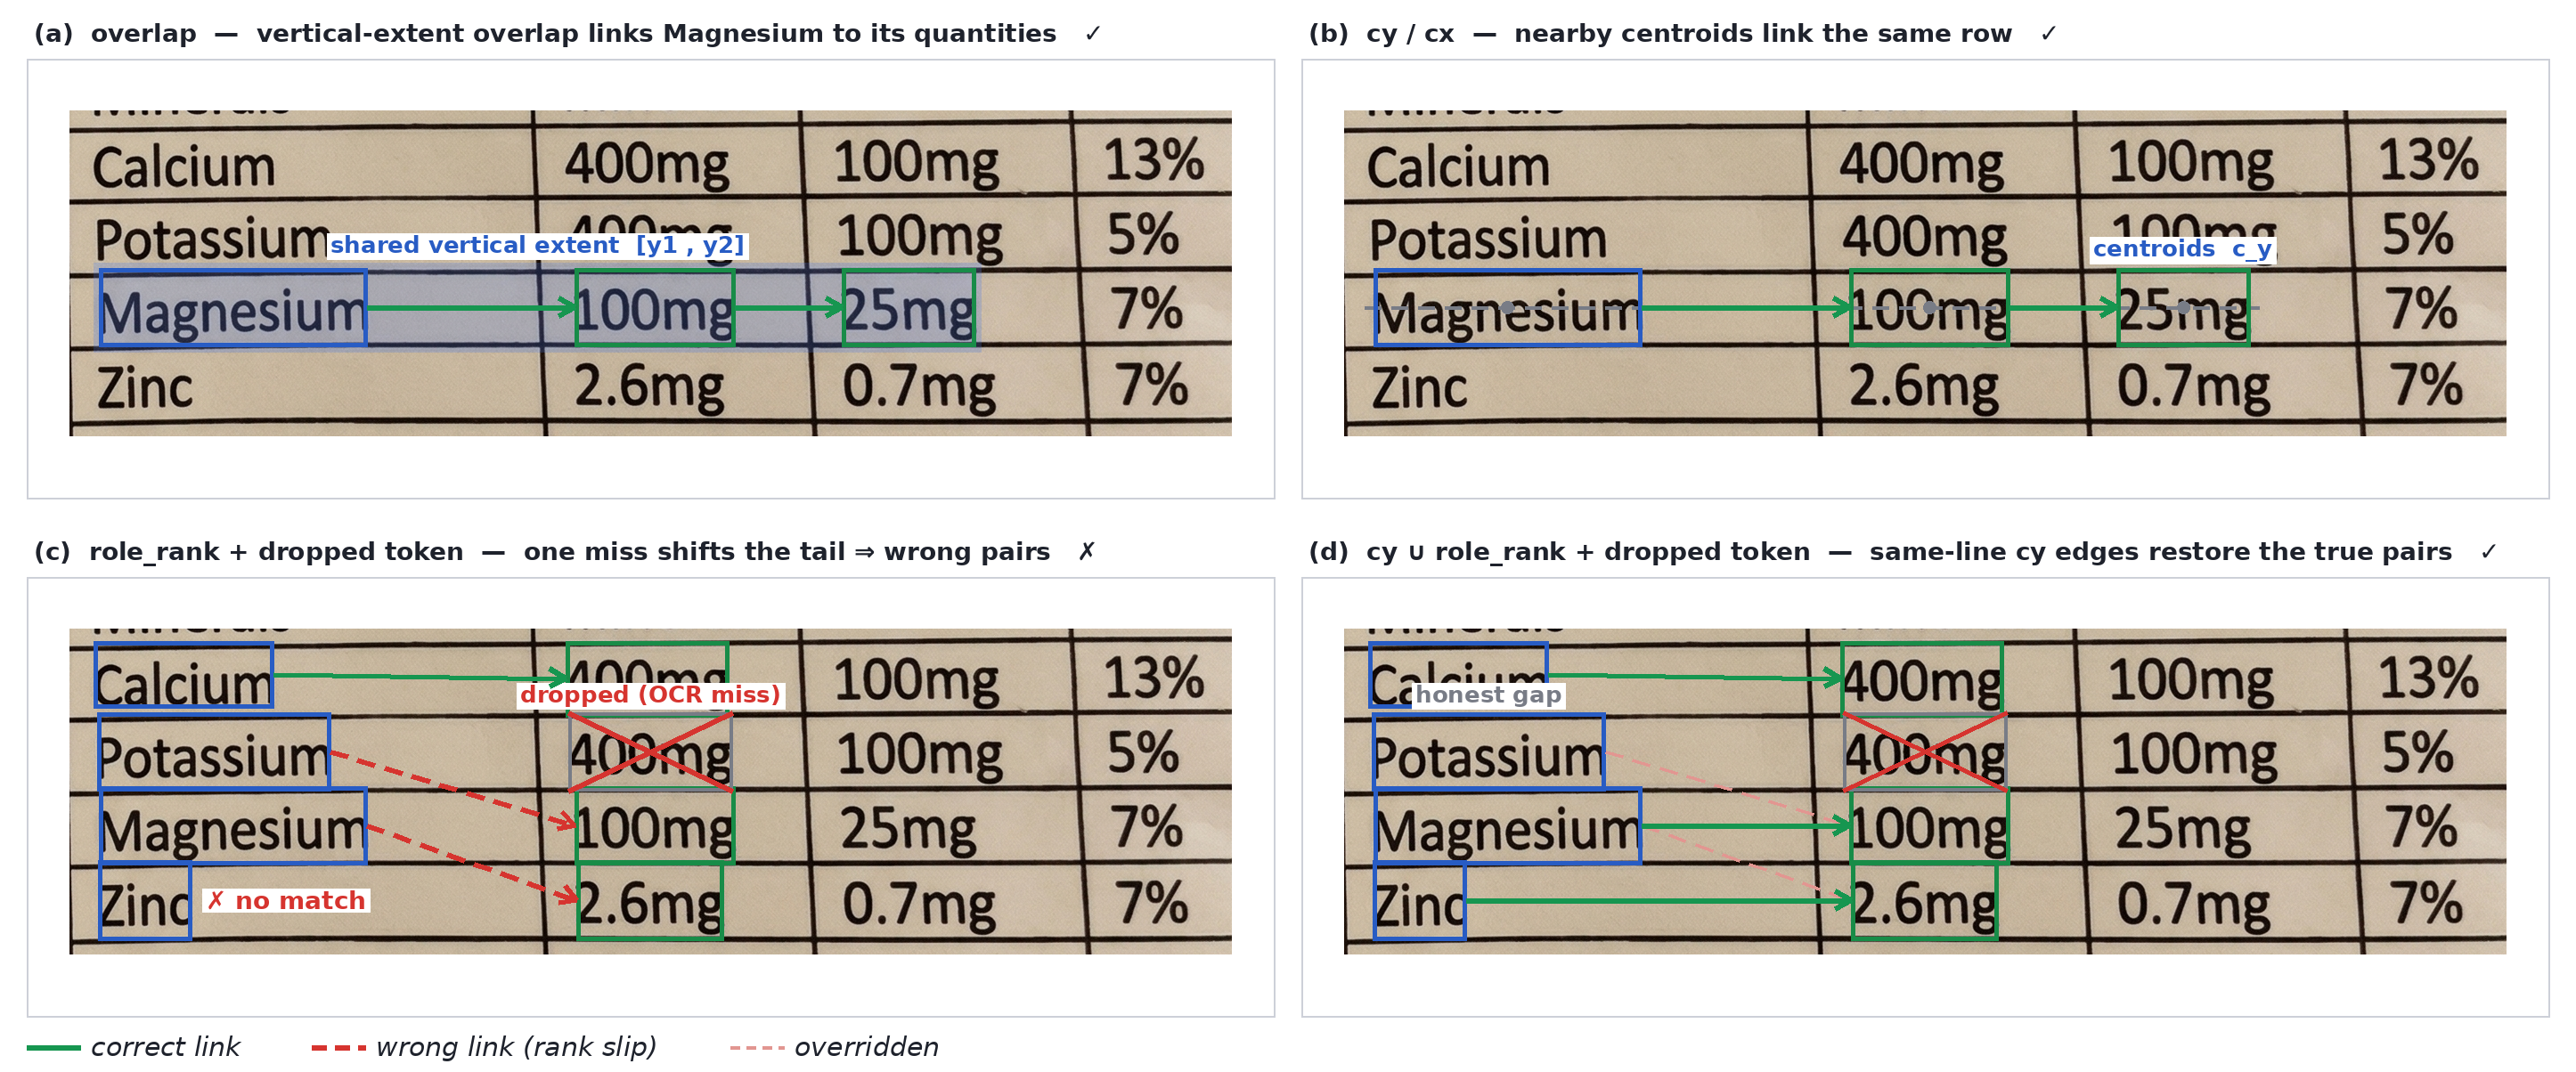
\includegraphics[width=\linewidth]{row_edge_over_image.png}%
  }{%
    \fbox{\parbox[c][45mm][c]{0.92\linewidth}{\centering\itshape
      Row-edge modes on a real label placeholder. Replace with
      \mcode{row_edge_over_image.png}.}}%
  }
  \caption[Row-edge modes on a real label]{%
    The four row-edge modes on a real label (34.png), where OCR has dropped
    Potassium's 400\,mg value. This is the real-data version of
    Figure~\ref{fig:row-modes}. (a)~and~(b) use geometry and pair each nutrient
    with its own quantities. (c)~uses rank order, so the missing value shifts
    the rest and pairs the wrong numbers. (d)~adds the geometric edges on top of
    the ranks and fixes the pairs again. Green is a correct link, red is a wrong
    one, and pink is a rank link that geometry overrides.}
  \label{fig:row-modes-real}
\end{figure}

The last question is which edge-creation mode builds the best row edges
inside graph~v2. The four modes defined in Section~\ref{sec:graph-v2} are
compared: the two geometric modes \mcode{overlap} and \mcode{cy-cx}, the
structural mode \mcode{role_rank}, and the union \mcode{cy}\,$\cup$\,\mcode{role_rank}.
OCR, the classifier, and the rest of graph~v2 are held fixed, so only the
row-edge rule changes. The sweep is run on the embedding classifier, which
covers all four modes, and is confirmed on GLiNER, which covers the two
geometric modes.

Table~\ref{tab:edge-modes} ranks the modes by four-field F1.

\begin{table}[htbp]
  \centering
  \caption[Graph v2 edge modes ranked by 4F-F1]{Graph~v2 edge-creation
    modes ranked by four-field tuple F1, with OCR and classifier fixed.
    The embedding rows cover all four modes; the GLiNER rows confirm the
    two geometric modes. \mcode{overlap} is best in both. All runs use the
    same deterministic evaluator (zero model calls), so the scores are
    directly comparable.}
  \label{tab:edge-modes}
  \small
  \begin{tabular}{@{}llc@{}}
    \toprule
    \textbf{Classifier} & \textbf{Edge mode} & \textbf{4F-F1} \\
    \midrule
    Embedding & \mcode{overlap}                  & 0.4025 \\
    Embedding & \mcode{cy-cx}                     & 0.3860 \\
    Embedding & \mcode{cy}\,$\cup$\,\mcode{role_rank}     & 0.3190 \\
    Embedding & \mcode{role_rank}                 & 0.1320 \\
    \addlinespace
    GLiNER    & \mcode{overlap}                   & 0.4304 \\
    GLiNER    & \mcode{cy-cx}                      & 0.4135 \\
    \bottomrule
  \end{tabular}
\end{table}

The ranking is the same for both classifiers. The geometric \mcode{overlap}
mode is best, the centre-based \mcode{cy-cx} mode is close behind, and the
two modes that use ordinal rank are worse. The structural \mcode{role_rank}
mode is the weakest by a wide margin, at 0.1320, because a single missed or
fused token shifts the rank order and breaks the row alignment, as
explained in Section~\ref{sec:enrichment-rowviews}. The union
\mcode{cy}\,$\cup$\,\mcode{role_rank} is also below the geometric modes, because
adding the rank-based edges to the geometric ones brings in wrong row links
rather than new correct ones. Geometric row edges are therefore the right
choice, and \mcode{overlap} is used as the default edge mode in every
graph~v2 run in this chapter.

\begin{figure}[t]
  \centering
  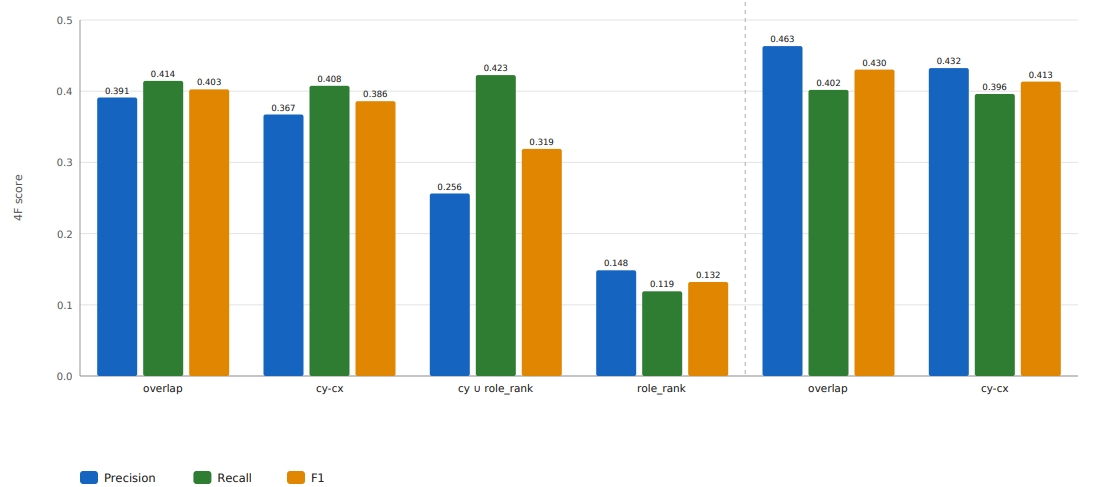
\includegraphics[width=1.15\linewidth,keepaspectratio]{edge_modes_bars.png}
  \caption[Graph v2 edge modes: precision, recall, and F1]{Four-field
    precision, recall, and F1 for the graph~v2 edge modes, with OCR and
    classifier fixed. The embedding sweep (left) covers all four modes; the
    GLiNER sweep (right) covers the two geometric modes. \mcode{overlap}
    has the highest F1 in both. The \mcode{cy}\,$\cup$\,\mcode{role_rank}
    mode has the highest recall in the embedding sweep but a much lower
    precision, showing that merging the rank-based edges adds tuples at the
    cost of precision; \mcode{role_rank} alone is weakest on all three
    metrics.}
  \label{fig:edge-modes-bars}
\end{figure}

% =====================================================================
%  6.7  CROSS-AXIS SYNTHESIS
% =====================================================================
\section{Cross-Axis Synthesis}\label{sec:exp-synth}

Each axis was settled on its own. Taken together, they show which choices
carried the result and which barely changed it. OCR stands apart from the
rest: PaddleOCR wins outright (Section~\ref{sec:exp-ocr}) and is used in
every run, so the questions that remain are the classifier and the
association engine, and those two pull against each other.

Figure~\ref{fig:effect-sizes} ranks the changes by how far each one moved
the four-field F1. Reading the text correctly matters most, and the switch
from EasyOCR to PaddleOCR is the largest jump of all. Next comes the move
from graph~v1 to graph~v2. The classifier moves the score least. So most of
the gain comes from reading the tokens and binding them with the better
graph; the classifier is a smaller adjustment on top.

\begin{figure}[t]
  \centering
  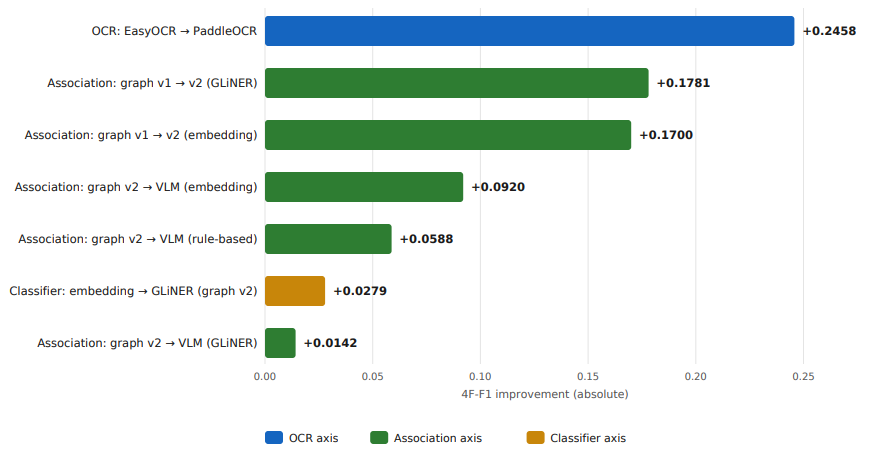
\includegraphics[width=1.15\linewidth,keepaspectratio]{effect_sizes.png}
  \caption[Effect of each pipeline change on 4F-F1]{Effect of each pipeline
    change on the four-field tuple F1. Each bar is the change from one
    substitution, with every other stage fixed. The OCR engine is the
    largest single factor, the move from graph~v1 to graph~v2 is next, and
    the classifier choice is the smallest.}
  \label{fig:effect-sizes}
\end{figure}

The runs also fall into three tiers, set by how much of the pipeline can be
inspected. In Tier~1 every stage is a rule or a graph, including the step
that turns tokens into tuples. Tier~2 keeps the upstream stages and swaps
only the binding step for a vision--language model. Tier~3 keeps no
structure at all: the image goes straight to a vision--language model and
the tuples come back. Table~\ref{tab:tiers} gives the best run in each.

\begin{table}[htbp]
  \centering
  \caption[Three interpretability tiers]{The three interpretability tiers
    and the best run in each. Tier~1 uses no black box at any stage.
    Tier~2 keeps the interpretable upstream stages and replaces only the
    association step with a vision--language model. Tier~3 hands the raw
    image to a vision--language model and reads the tuples directly from
    its output. The score is four-field tuple F1.}
  \label{tab:tiers}
  \small
  \begin{tabular}{@{}llc@{}}
    \toprule
    \textbf{Tier} & \textbf{Best run} & \textbf{4F-F1} \\
    \midrule
    Tier~1 --- fully interpretable                 & E2-C (GLiNER, graph~v2)            & 0.4304 \\
    Tier~2 --- interpretable upstream, VLM assoc.   & E3-EMB-VLM (embedding, VLM assoc.) & 0.4945 \\
    Tier~3 --- fully black-box end-to-end          & E4 (end-to-end VLM)                & 0.3597 \\
    \bottomrule
  \end{tabular}
\end{table}

How the tiers rank is the main result of the chapter. Tier~2 comes
first---E3-EMB-VLM reaches 0.4945, with the interpretable upstream stages
feeding a model that only has to bind. The fully interpretable Tier~1 run,
E2-C, follows at 0.4304. Last is the black-box Tier~3 run, E4, at 0.3597.
Two points stand out. The structured pipeline beats the raw model by about
seven points, so shaping the problem before binding any field clearly pays
off. And the only runs that beat the interpretable pipeline keep their
upstream stages and change one step, so the extra points come from the
binding step alone---and they cost interpretability.

Different goals favour different runs, as Table~\ref{tab:best-by-objective}
shows.

\begin{table}[htbp]
  \centering
  \caption[Best configuration by objective]{Best configuration for each
    objective, over all runs in this chapter. The metric shown is the one
    the objective names; all values are four-field tuple scores.}
  \label{tab:best-by-objective}
  \small
  \begin{tabular}{@{}llc@{}}
    \toprule
    \textbf{Objective} & \textbf{Best configuration} & \textbf{Score} \\
    \midrule
    Highest tuple F1 (overall)       & E3-EMB-VLM (embedding, VLM assoc.) & 0.4945 \\
    Highest tuple F1 (interpretable) & E2-C (GLiNER, graph~v2)            & 0.4304 \\
    Highest tuple precision          & E3-EMB-VLM (embedding, VLM assoc.) & 0.6054 \\
    Highest tuple recall             & E2-A (rule-based, graph~v2)        & 0.4238 \\
    \bottomrule
  \end{tabular}
\end{table}

E3-EMB-VLM has the best F1 and the best precision. Recall peaks with E2-A,
the rule-based graph run, which recovers the most correct tuples but admits
enough wrong ones to fall well behind on precision. For a fully
interpretable system, E2-C is the pick. No run leads on every measure, so
the choice follows whatever the task values most.

The classifier and the association engine interact in a tidy way. Put
GLiNER with the graph and the interpretable score is best: GLiNER is
precise, so few wrong candidates ever reach the graph (E2-C, 0.4304). Put
the embedding classifier with the vision--language model and the overall
score is best: of the learned classifiers it finds the most nutrients, and
the model discards the wrong bindings its extra candidates would otherwise
produce (E3-EMB-VLM, 0.4945). Either way, the rule-based classifier sits in
the middle. There is no single best classifier; the right one depends on
what does the binding.

\begin{figure}[t]
  \centering
  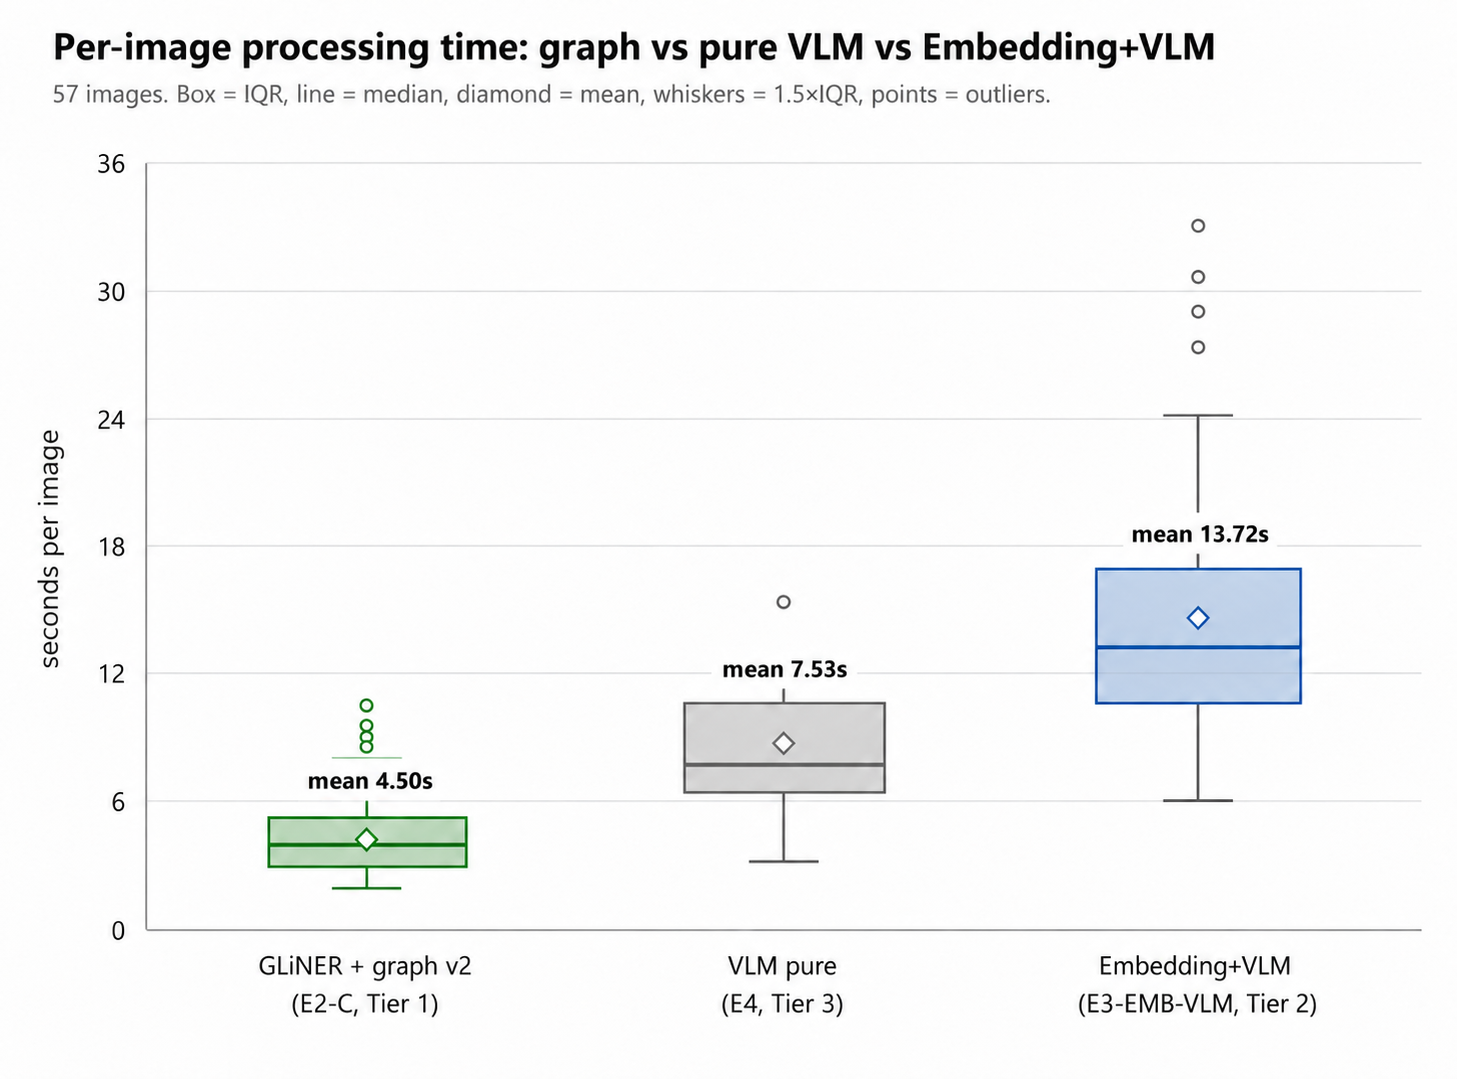
\includegraphics[width=\linewidth,keepaspectratio]{per_image_runtime.png}
  \caption[Per-image processing time by tier]{Per-image processing time for
    the three tiers, over the 57 test images. The box is the interquartile
    range, the line the median, and the diamond the mean. The interpretable
    pipeline (E2-C) is fastest, the end-to-end model (E4) sits in between,
    and the embedding-plus-VLM hybrid (E3-EMB-VLM) is the slowest.}
  \label{fig:runtime}
\end{figure}

Cost separates the runs as sharply as score does.
Figure~\ref{fig:runtime} gives the per-image time for the three tiers. The
interpretable pipeline is fastest, at a mean of 4.50 seconds, because it
never calls the model. The pure end-to-end run sits in the middle at 7.53
seconds. Slowest is the embedding-plus-VLM hybrid at 13.72 seconds---about
three times the interpretable pipeline---since it runs the full upstream
pipeline and then adds a model pass. The best-scoring run is therefore also
the most expensive. That model pass is likewise the step that cannot be
read back, where the graph binds by a rule one can inspect. So the points
won by VLM-association are paid three ways: in runtime, in compute, and in
interpretability. Which configuration fits depends on the time budget and
on whether the binding step must be inspectable.
Section~\ref{sec:exp-error} turns to the errors that remain in every
configuration and where they begin.

% =====================================================================
%  6.8  ERROR ANALYSIS
% =====================================================================
\section{Error Analysis}\label{sec:exp-error}

This section looks at where tuples are lost. It uses the best interpretable
run, E2-C (GLiNER with graph~v2), because every stage in it is a rule or a
graph and the losses can be followed step by step; the runs that bind with
the vision--language model hide that step inside a model that cannot be read
back. The losses traced here sit before the binding step, so the runs that
share the same OCR and classifier carry them too.

Table~\ref{tab:funnel} follows the 866 gold tuples through the run. The
nutrient is matched for 552 of them, and 348 of those come out fully
correct. Two losses remain. The larger one is the 314 tuples whose nutrient
is never matched---about a third of the gold set is gone before any field is
attempted. The smaller one is the 204 tuples that match on the nutrient but
get at least one field wrong. Separately, 199 of the 751 predicted tuples
match no gold nutrient at all, and these drag precision down.

\begin{table}[htbp]
  \centering
  \caption[Where the gold tuples go]{Where the gold tuples go under the best
    interpretable run, E2-C (GLiNER, graph~v2), on the full test set (866
    tuples, 57 images) and the reduced set (820~tuples, 55~images) with
    images 15 and 67 removed. A tuple is nutrient-matched when its nutrient
    is paired with a prediction; the fully correct ones have all four fields
    right. The false positives are predicted tuples that match no gold
    nutrient. The analysis in this section reads the full set.}
  \label{tab:funnel}
  \small
  \begin{tabular}{@{}lcc@{}}
    \toprule
    \textbf{Outcome} & \textbf{Full (866)} & \textbf{Reduced (820)} \\
    \midrule
    Gold tuples                            & 866 & 820 \\
    Nutrient matched                       & 552 & 543 \\
    \quad fully correct (all four fields)  & 348 & 339 \\
    \quad one or more fields wrong         & 204 & 204 \\
    Nutrient not matched (recall loss)     & 314 & 277 \\
    \addlinespace
    Predicted tuples                       & 751 & 742 \\
    \quad false positives (no gold match)  & 199 & 199 \\
    \midrule
    Four-field precision                   & 0.4634 & 0.4569 \\
    Four-field recall                      & 0.4018 & 0.4134 \\
    Four-field F1                          & 0.4304 & 0.4341 \\
    \bottomrule
  \end{tabular}
\end{table}




The 204 partial failures do not fall evenly on the four fields. After the
nutrient is matched, context is read most reliably and quantity least: the
per-field accuracies are 87.9, 83.2, and 76.3 percent for context, unit,
and quantity (Section~\ref{sec:exp-classifier}). Quantity is the weak field,
wrong on 131 of the 552 matched tuples. Reading a number and tying it to the
right nutrient is simply harder than reading a short unit or a column
header.

Three patterns produce most of these losses. Some images defeat the OCR
outright: on 68.jpeg the text returns corrupted, and 67.jpeg is a
pharmaceutical label the engine reads poorly, so their 34 and 4 gold tuples
fall at the nutrient stage. Others defeat the table logic rather than the
OCR---15.PNG lays its 42 values out in running paragraphs instead of a
table, and only the paragraph fallback recovers any of them.
(Images 15 and
67 are the two later removed from the primary test set, as noted in
Chapter~\ref{chap:evaluation};they are discussed here because this analysis
is run on the full 866-tuple set.) The rest is the
quantity misalignment behind the weak quantity field. The value columns are
separated and labelled in the enrichment stage, and on dense tables that
place two value columns side by side, as 118.jpeg and 119.jpeg do across
their 40 gold tuples, that stage can place a value in the wrong column---so
a per-serving number is bound where the per-100\,g number belongs.

Two limits therefore bound the interpretable pipeline: the recall ceiling
set by what the OCR and classifier recover, and the column misalignment that
mis-binds quantities on dense tables. Both arise before the binding step.
The graph cannot repair either, since it binds from the columns and tokens
it is handed. The vision--language model lifts precision---with the
classifier held fixed, swapping the graph for the model barely moves recall
(embedding, 0.4145 to 0.4180)---but the nutrients missed upstream stay
missed. Section~\ref{sec:exp-summary} brings the chapter's findings
together.


% =====================================================================
%  DISTANCE-BASED LINKING VALIDATION
%  (placement: new section after Section~\ref{sec:exp-error} (Error Analysis),
%   i.e. the new 6.9, with Summary of Findings becoming 6.10)
%  Figure file: fig_below_above_split.png  (the two-panel below/above chart)
% =====================================================================
\section{Distance-Based Linking Validation}\label{sec:exp-distance}

Section~\ref{sec:exp-edge} showed that geometric row edges work better than
rank-based ones. This section checks the same idea in a simpler way. When we
join a nutrient to a quantity, how far apart are their boxes on the label?
And can this distance tell a good link from a bad one? The test uses the
PaddleOCR front-end, and it does not change any score in this chapter.

First, we need to say which pairs are allowed. We use the same idea as the
error analysis (Section~\ref{sec:exp-error}): the OCR usually loses
quantities, but it reads nutrient names well. Suppose only quantities are
lost. Then the list of nutrients stays complete and in order. When a quantity
is lost, the quantities under it move up. So a nutrient can never take a
quantity that comes before it. It can only take its own quantity or one that
comes later. In rank terms, a nutrient at rank~$k$ is joined to every quantity
at rank~$k$ or larger, where rank means the top-to-bottom order. If no
quantity is lost, this is just rank~$k$ to rank~$k$.

For each pair, we draw a vector from the middle of the nutrient box to the
middle of the quantity box. The average is then worked out for each image on
its own: we take all the vectors on that one image and find their average, so
every image has its own average vector. Inside an image, we also do this column
by column, so a per-100\,g column and a per-serving column are not mixed. Every vector is then longer or shorter
than this average. Figure~\ref{fig:displacement-belowabove} shows the two
counts for each label. On the 55 labels, 4{,}605 pairs were made. Almost half
are below the average (2{,}119, or 46\%), and a little more than half are above
it (2{,}486, or 54\%). Some labels have fewer than two quantities. Then no
column can be made, so the label is left out. These are the empty places in the
figure (78.jpeg, 111.jpeg and 112.jpeg; 15.png and 67.jpeg were removed
earlier).

\begin{figure}[t]
  
  \makebox[\linewidth][c]{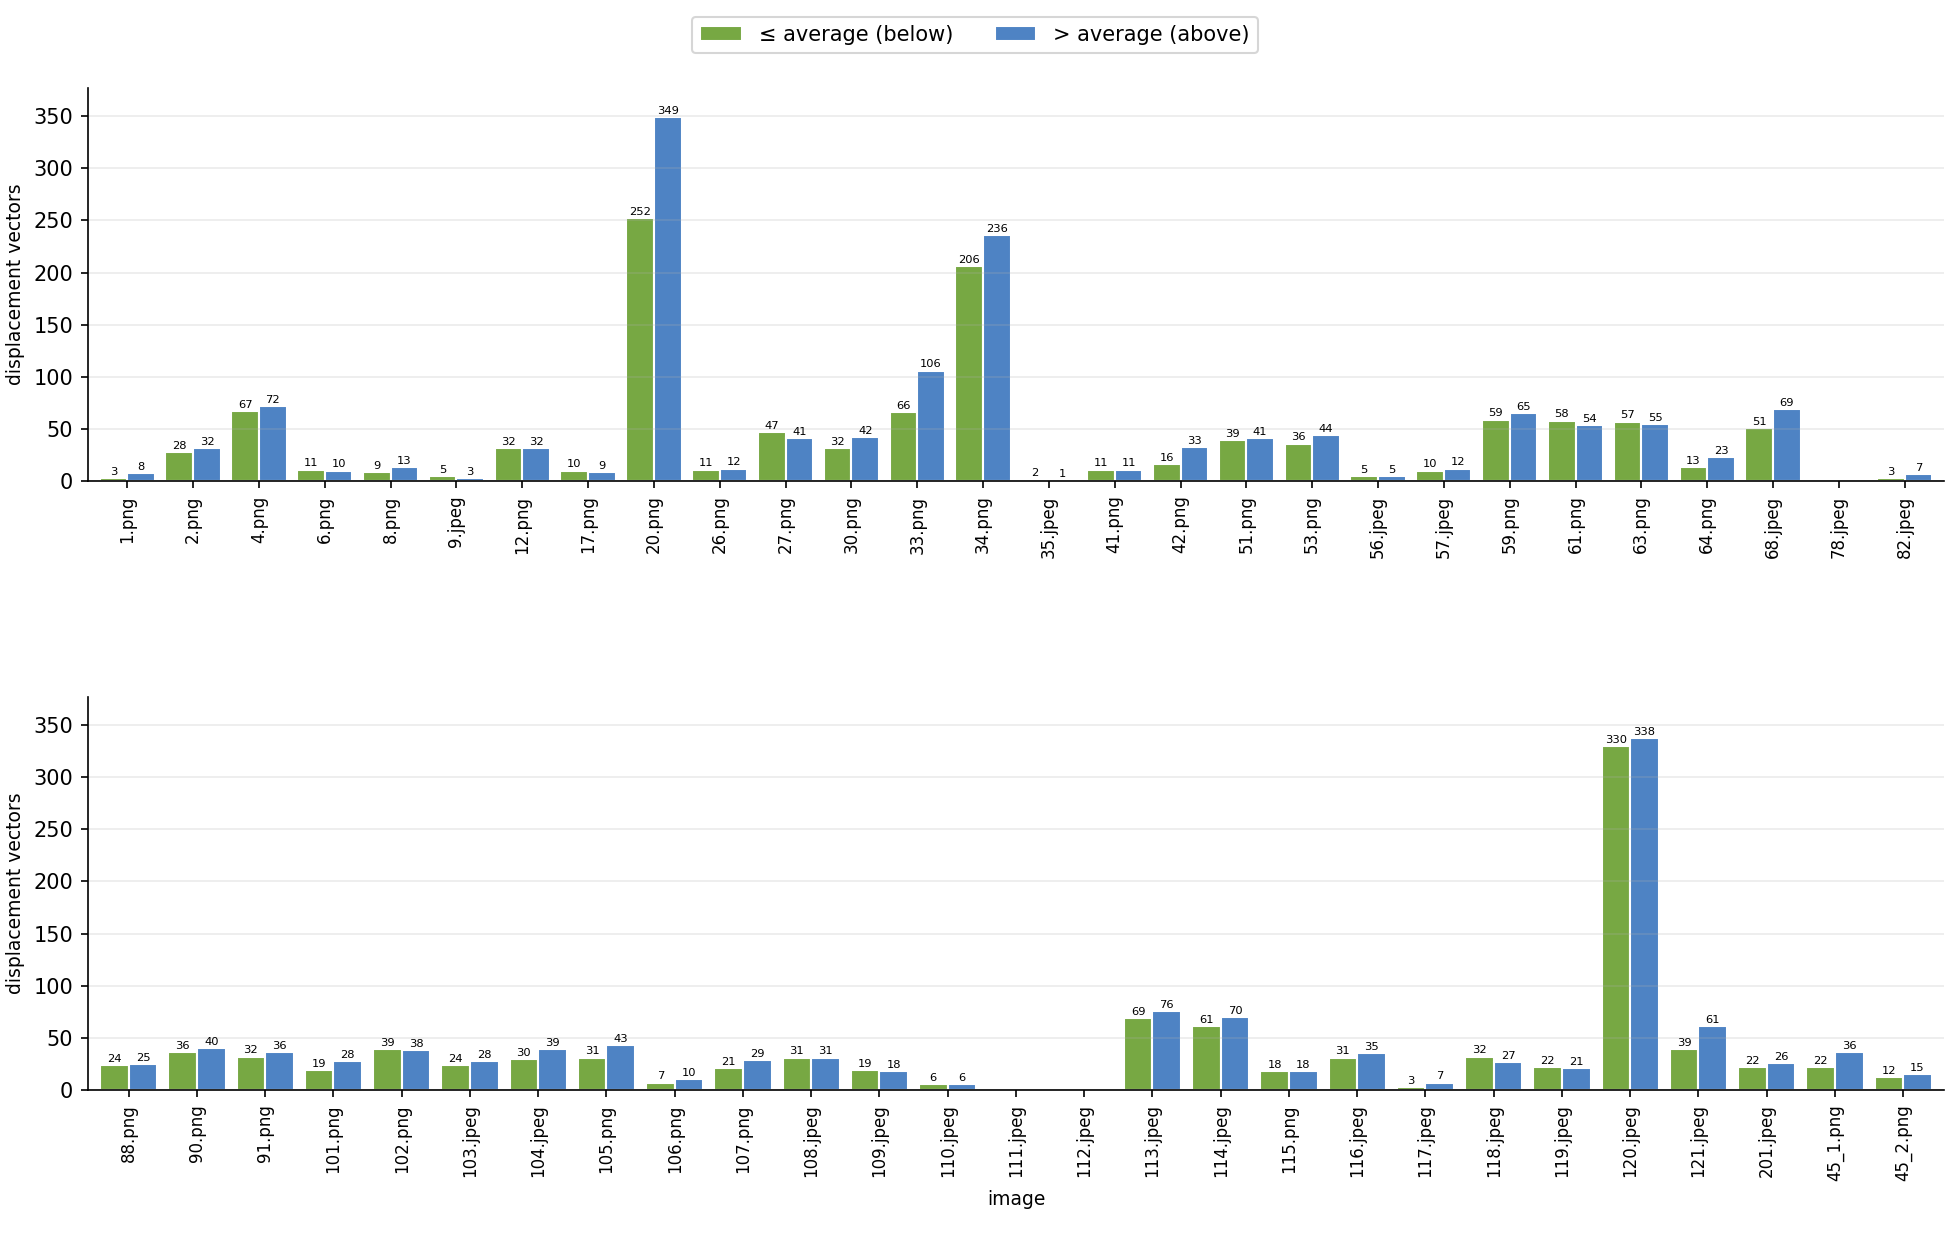
\includegraphics[width=1.4\linewidth,keepaspectratio]{fig_below_above_split.png}}
  \caption[Displacement vectors below and above the image average]{%
    For each label, the number of vectors that fall below (green) and above
    (blue) that label's own average vector. A pair is one possible
    nutrient--quantity link, measured from the middle of the nutrient box to
    the middle of the quantity box. Empty places are labels with too few
    quantities to make a pair. The 55 labels are shown in two rows so they are
    easier to read.}
  \label{fig:displacement-belowabove}
\end{figure}

Two things come out of this. First, real links sit in a steady place. On every
label the horizontal part of the average vector is large, because the quantity
is to the right of the name, and the vertical part is small. So a real pair has
a short and stable gap. This says the same thing as Section~\ref{sec:exp-edge},
but without the tuple score: what keeps a link together is position, not order.
Second, the distance finds many links but cannot pick between them. On the two
fields it can check---the nutrient and its value---the below-average pairs
cover 366 of the 866 gold links (42\%). This is close to the 421 (49\%) that
the full pipeline with the \mcode{overlap} edge mode reaches on the same two
fields (Section~\ref{sec:exp-error}).
But the split in Figure~\ref{fig:displacement-belowabove} is almost even. A
real link is about as likely to be above the average as below it. So the
distance only suggests good pairs; it does not choose them. This is why the
association stage joins them with the geometric edges of
Section~\ref{sec:graph-v2}, and not with a simple distance rule. One last
point: this measure cannot find missing values. A token that is never read has
no box, so it has no vector, and a lost quantity leaves no mark here at all.


% =====================================================================
%  6.9  SUMMARY OF FINDINGS
% =====================================================================
\section{Summary of Findings}\label{sec:exp-summary}

The chapter answered five questions by ablation, changing one stage at a
time. This section collects the answers.

OCR matters most. PaddleOCR beats EasyOCR on every field, and the gap is in
the values rather than the names: quantity, unit, and context each rise by
twenty-five to thirty points, while nutrient detection barely moves. The
four-field F1 climbs from 0.1773 to 0.4231 on the OCR change alone, so
PaddleOCR is used in every other run.

The association engine is the next-largest factor, and its design is where
the interpretable result is made. Graph~v2 nearly doubles the four-field F1
of graph~v1 for both learned classifiers, and the gain is structural: it
shows on the multi-context labels, the ones with more than one value column,
where graph~v1 cannot keep the columns apart. Inside graph~v2, geometric row
edges are the right choice---the \mcode{overlap} mode wins, the rank-based
modes are much weaker, and adding rank edges to the geometric ones only
brings in wrong links. The classifier is the smallest factor. It acts only
through nutrient detection, since the shared cascade reads quantity, unit,
and context the same way whichever classifier is used; among the zero-shot
options GLiNER gives the best interpretable tuple score, 0.4304, with no
curated lexicon.

That run, E2-C, is the best fully interpretable pipeline and the chapter's
main result. Replacing only the binding step with a vision--language model
raises the score further, to 0.4945, by lifting precision while recall
holds---and with the model doing the binding, the embedding classifier
overtakes GLiNER, reversing the order seen on the graph. Both of these beat
a vision--language model run end to end, which reaches only 0.3597, so
structuring the problem before any field is bound is worth more than handing
the whole task to one model. The extra points from the model are paid for in
interpretability and in time: the interpretable pipeline runs in about four
and a half seconds per image, the hybrid in about fourteen.

Two limits bound all of these configurations. About a third of the gold
tuples are lost because the nutrient is never read, a ceiling set by the OCR
and the classifier; and quantity is the weakest field, mis-bound on dense
tables where two value columns sit side by side. Both arise before the
binding step, so they pass through every run. What they suggest for the
design, and the work that remains, is taken up in the following chapter.